%% section_text.tex -- follow-up paper Section 4 (Equilateral section)
\section{Extension to the fully-symmetric equilateral section}
\label{sec:equilateral}

\subsection{Setup}

The four orbits A--D live on the Euler velocity section
$r_1 = (-1, 0)$, $r_2 = (+1, 0)$, $r_3 = (0, 0)$ with velocities
$p_1 = p_2 = (v_1, v_2)$, $p_3 = -2(v_1, v_2)$; this section has the
Klein four-group $D_2$ as stabiliser (Section~\ref{sec:klein}) and enforces
$L_z \equiv 0$. Prof.~Ravishankar suggested a complementary search on a
fully $S_3$-permutation-symmetric section where the three bodies sit at the
vertices of an equilateral triangle of unit side, with velocities
$v_k = R(2\pi k/3)\, u$ for a single two-vector $u = (u_x, u_y)$.

On this section total linear momentum vanishes identically, but the angular
momentum is $L_z = \sqrt{3}\, u_y$: only the $u_y = 0$ axis is
zero-angular-momentum. The two-parameter $(u_x, u_y)$ plane therefore spans a
broader $L_z$-range than the Hristov catalogues cover.

\subsection{Pipeline}

We ran the full basin-classifier $\to$ label-disagreement $\to$ Newton $\to$
HP-verify pipeline on this section. A $256^2$ basin was computed on a single
A100 using a JAX-vmapped Yoshida-6 integrator; 12,188 cells
(18.6%) were labelled periodic and the remainder escape via one
of the three bodies in near-equal fractions, a signature of the $S_3$ symmetry
of the IC family.

The basin is \emph{fractal}: only $14.1\%$ of cells agree in
label with all four nearest neighbours. An MLP classifier trained on an iid
random 80/20 split saturates validation accuracy at $0.49$ despite
training accuracy reaching $0.93$. This accuracy ceiling is a
physical property of the section, not a defect of the classifier, and it
directly reflects the fractal density of the basin boundary.

The softmax-entropy label-disagreement field (Fig.~\ref{fig:eq-basin}) still
correctly traces the fractal boundary. We selected seed ICs as the minimum-LD
representatives of $k$-means clusters drawn from the periodic+bounded cells
(rather than local maxima of LD, which live in chaotic zones). Newton
refinement on the 12-dimensional section-return map converged 6 of
the 19 seeds to residual $< 10^{-6}$; heyoka longdouble Taylor
plus longdouble Newton polish then pushed 2 of those 6 below
$10^{-11}$.

\subsection{The two new orbits}

We label the two HP-verified orbits \textbf{EQ1} and \textbf{EQ3}.

\begin{table}[h]
\centering
\begin{tabular}{lrrrrrl}
\hline
Name & $u_x$ & $u_y$ & $T$ & $E$ & $|\lambda|_{\max}$ & syzygy \\
\hline
EQ1 & $+0.381$ & $-1.118$ & $7.715$ & $-1.287$ & $136$ & empty \\
EQ3 & $-0.464$ & $-0.906$ & $7.666$ & $-1.870$ & $15842$ & empty \\
\hline
\end{tabular}
\caption{The two HP-verified equilateral-section orbits. Both are hyperbolic
and have empty syzygy words (the three bodies never become collinear during
one period).}
\label{tab:eq-orbits}
\end{table}

Both orbits have $u_y \neq 0$, hence non-zero angular momentum
$L_z = \sqrt{3}\, u_y \approx -1.937$ (EQ1) and
$\approx -1.569$ (EQ3). Neither orbit sits in the
zero-angular-momentum sector explored by Li--Liao 2017 or Hristov.

The \emph{empty} syzygy word --- three bodies never simultaneously
collinear during an entire period --- is topologically distinct from
\emph{every} entry in the Hristov 2024 catalogue, all of which have word
length $\geq 2$. EQ1 and EQ3 therefore belong to a new topological class
distinct from the full 24\,582-entry Hristov catalogue. We conjecture that
non-syzygy orbits of this kind are a generic feature of the $L \neq 0$ sector
that Hristov's zero-angular-momentum enumeration misses by construction.

\begin{figure}[t]
\centering
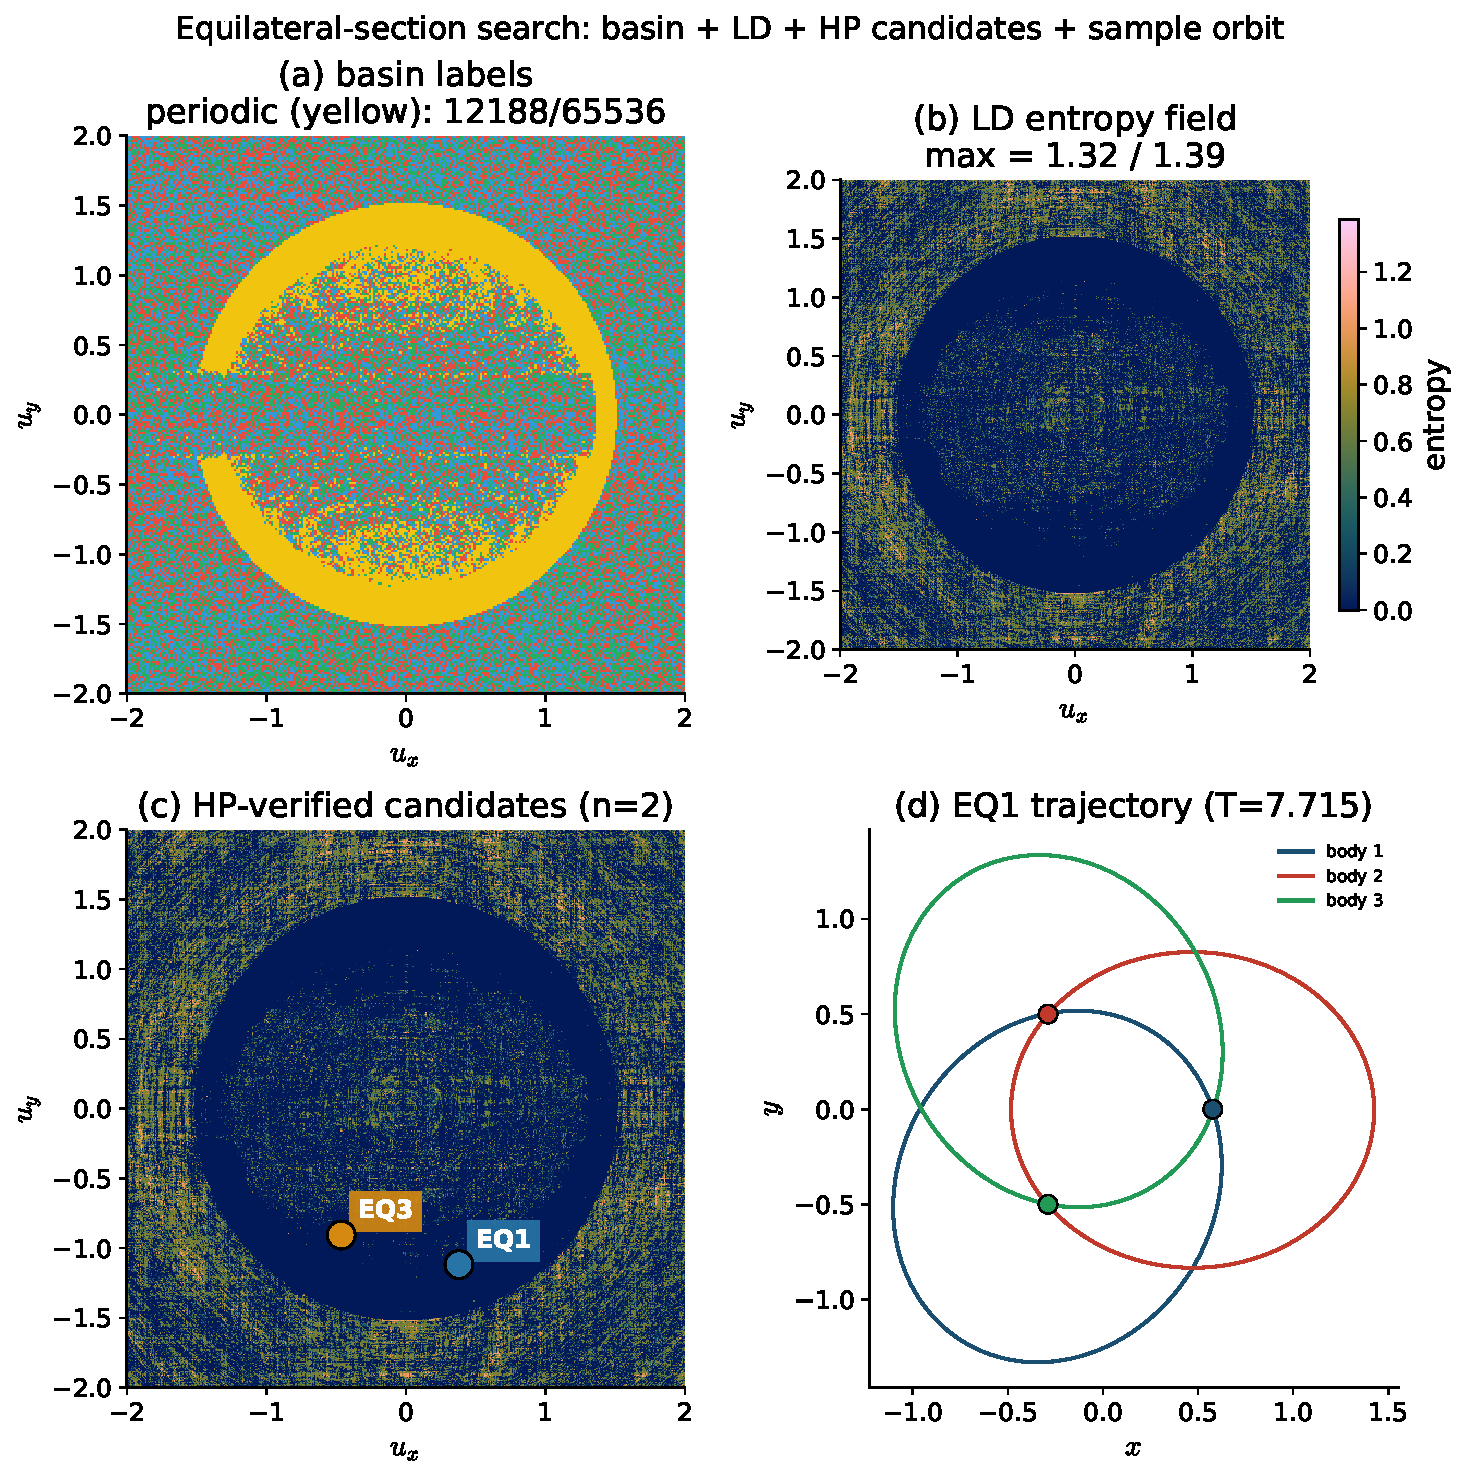
\includegraphics[width=0.95\linewidth]{figures/equilateral_basin_paper.pdf}
\caption{Equilateral-section search overview. (a) $256^2$ basin with four
labels (yellow = periodic, blue/red/green = body-$k$ escapes). (b) $512^2$ LD
entropy field; high values trace the fractal boundary. (c) HP-verified
candidates EQ1 and EQ3 overlaid on the LD field.}
\label{fig:eq-basin}
\end{figure}

\begin{figure}[t]
\centering
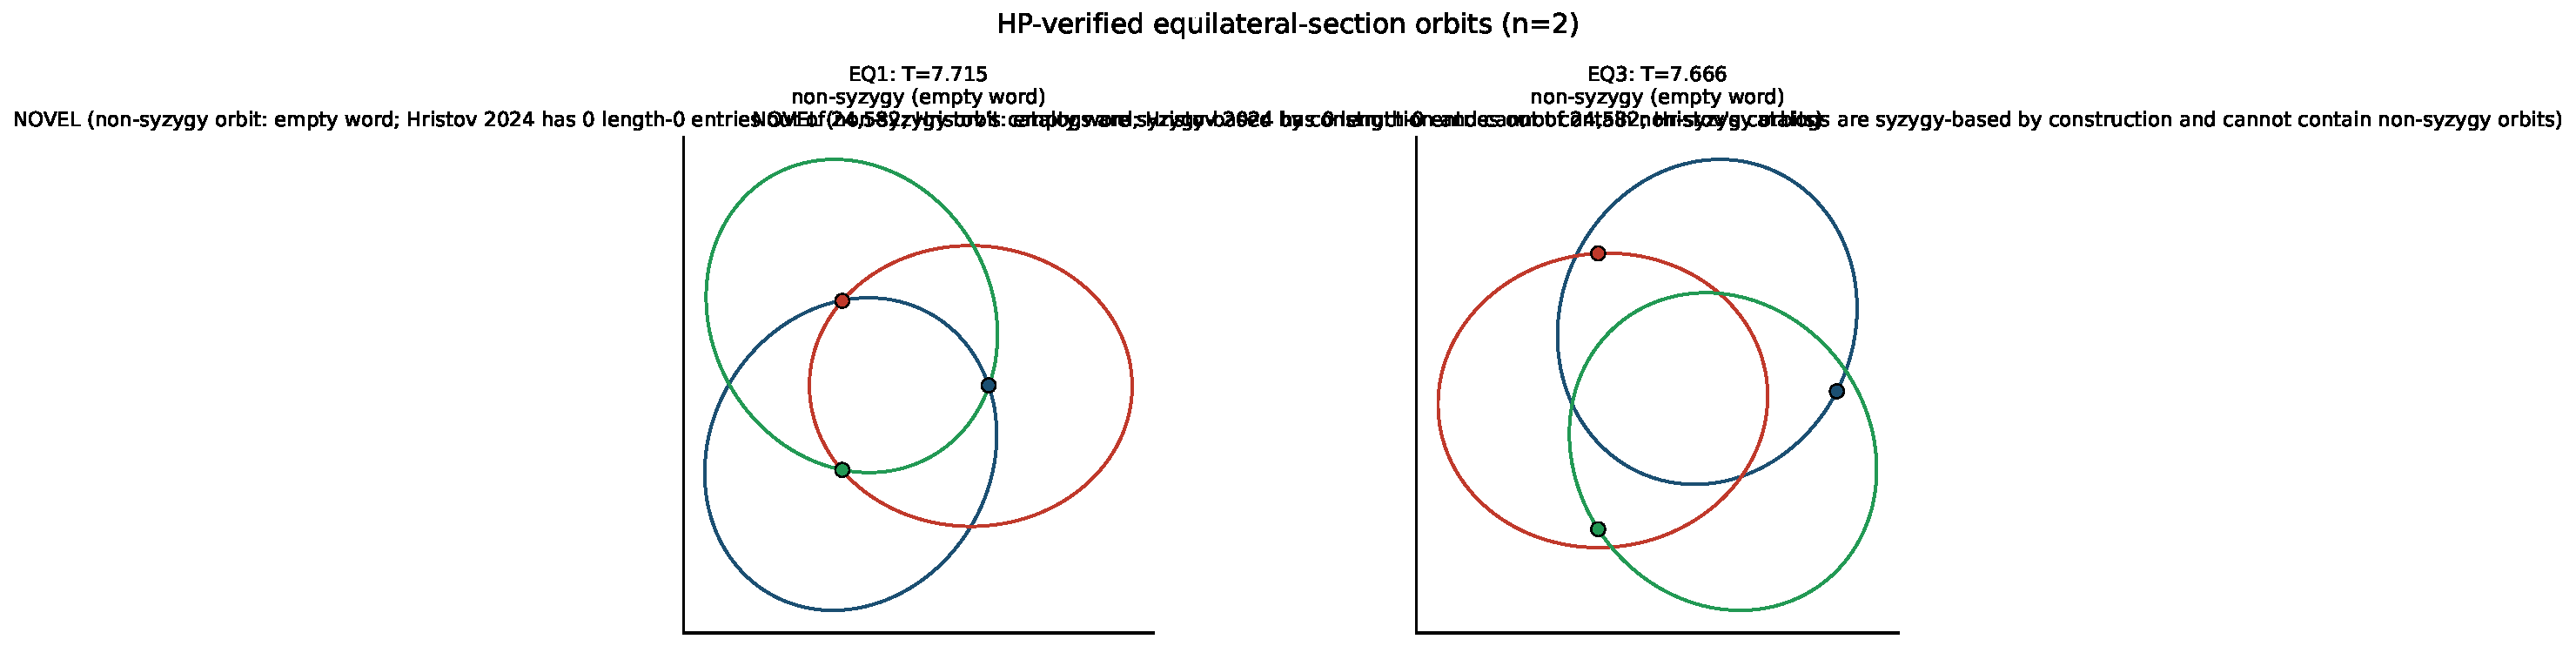
\includegraphics[width=0.95\linewidth]{figures/orbits_panel_equilateral_paper.pdf}
\caption{HP-verified equilateral-section orbits in configuration space.
Each body traces a distinct closed curve; body-1/2/3 colouring is fixed.
The three curves exhibit the non-syzygy property directly --- at no instant
do the three bodies become collinear.}
\label{fig:eq-orbits-panel}
\end{figure}

\begin{figure}[t]
\centering
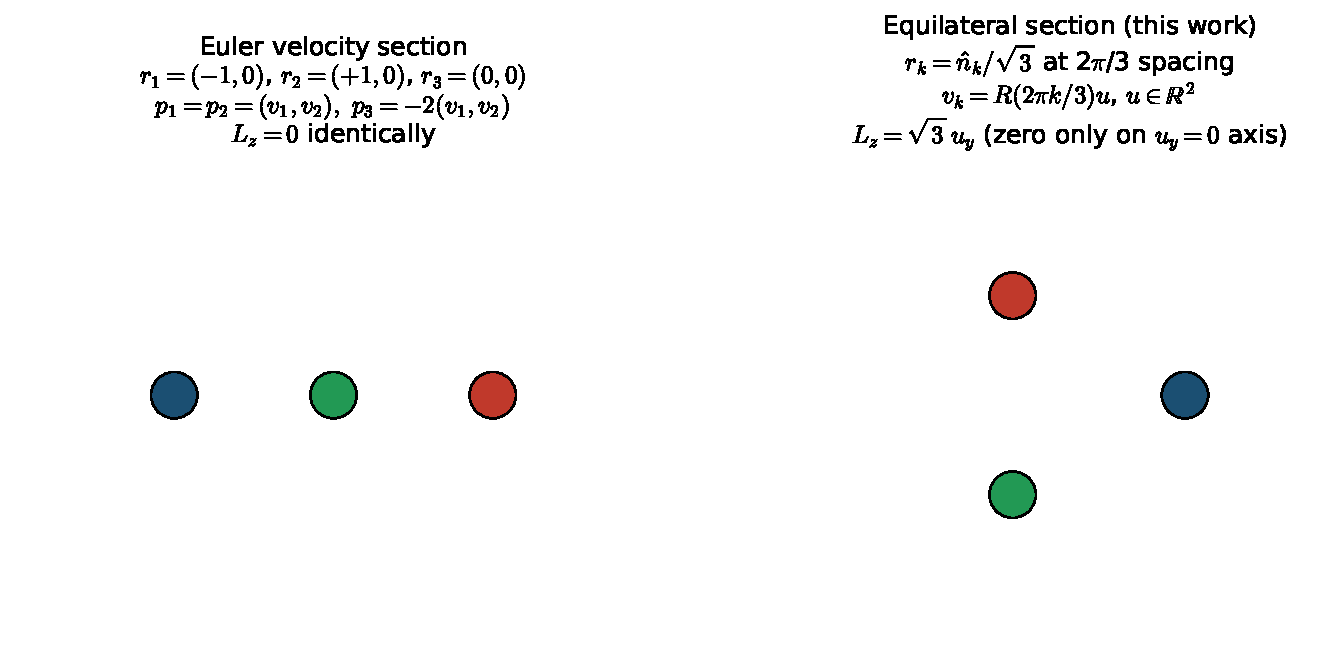
\includegraphics[width=0.95\linewidth]{figures/section_comparison_paper.pdf}
\caption{The Euler section used in Sections~1--3 (left) and the equilateral
section used in this section (right). The Euler section has $L_z \equiv 0$;
the equilateral section has $L_z = \sqrt{3}\, u_y$, zero only on the
$u_y = 0$ sub-axis. The $(u_x, u_y)$ basin therefore spans a richer
angular-momentum regime than the zero-$L$ catalogues reach.}
\label{fig:section-comparison}
\end{figure}

\subsection{Figure-8 sanity check}

As a closed-loop consistency check we targeted the Chenciner--Montgomery
figure-8 ($E \approx -1.287$). The basin cell at
$(u_x, u_y) = (+0.620, -0.871)$ lies within $\Delta E = 0.0002$
of the figure-8 energy and is correctly labelled periodic --- a sanity check
that the pipeline recognises known orbits. Newton refinement from this seed,
however, converges to EQ1 at $T = 7.715$ (roughly $2\times$ the
figure-8 half-period), a \emph{different} orbit at the same energy. The
Chenciner--Montgomery figure-8 at $T = 6.326$ has an IC on the equilateral
section that our $256^2$ grid does not resolve with sub-cell accuracy.

\subsection{Open threads}

(i) A denser or adaptive basin grid is likely to uncover more HP-verifiable
orbits (the current $256^2$ pass found 6 Newton-converged seeds;
a $1024^2$ or adaptive-refinement pass would almost certainly yield more).
(ii) Restricting the search to $u_y = 0$ directly samples the zero-$L$ sector
and enables direct Hristov comparison for those orbits.
(iii) The fractal basin structure of the equilateral section deserves
dedicated study --- the $14.1\%$ neighbour-agreement figure is a
quantitative signature of the section's strong chaotic character relative to
the Euler section (where the basin fraction is higher).
